\documentclass[a0,final]{a0poster}
%%%Load packages
\usepackage{multicol} 			%3-column layout
\usepackage[left=2cm,right=2cm,bottom=0cm,top=0cm]{geometry}			%Reset margins
\usepackage{mathpazo}			%Load palatino font & pazo math
\usepackage{color}				%Needed for colour boxes & coloured text


\usepackage{graphicx}     		%Needed to import images


\DeclareGraphicsExtensions{.pdf,.png,.jpg}

\graphicspath{ {./images/} }




%%%Define colours and lengths
\definecolor{headingcol}{rgb}{1,1,1}			%Colour of main title
\definecolor{boxcol}{rgb}{0.7,0.2,0.2}		%Edge-colour of box and top banner
\fboxsep=1cm							%Padding between box and text
\setlength{\columnsep}{2cm}				%Set spacing between columns

%%%Format title
\makeatletter							%Needed to include code in main file
\renewcommand\@maketitle{%
\null									%Sets position marker
{
\color{headingcol}\sffamily\VERYHuge		%Set title font and colour
\@title \par}%
\vskip 0.6em%
{
\color{white}\sffamily\large				%Set author font and colour
\lineskip .5em%
\begin{tabular}[t]{l}%
\@author
\end{tabular}\par}%
\vskip 1cm
\par
}
\makeatother

\title{BA Scale Free Networks}

\author{Dalwinder Bagdi, Tanvi Bhardwaj, Ankeet Dhanji, Dani Grayston, Alexandru Stoenescu \& Robert Al White\\
University of Manchester - Group 5}

\begin{document}

\hspace{-3cm}								%Align with edge of page, not margin
\colorbox{boxcol}{							%Coloured banner across top
\begin{minipage}{1189mm}					%Minipage for title contents
\maketitle
\end{minipage}}
\vspace{1cm}

\begin{multicols}{3}							%Use 3-column layout
\raggedcolumns							%Don't stretch contents vertically

%%%Column1
\section*{Introduction}
Lorem ipsum dolor sit amet, consectetuer adipiscing elit. Ut dui. Vivamus ullamcorper. Pellentesque metus dui, facilisis nec, aliquet ut, ultrices quis, ipsum. Mauris semper venenatis nunc. Nunc et leo. Morbi quis tortor quis ipsum rhoncus faucibus. Praesent nunc. Aliquam justo. Nullam vitae leo. Nam imperdiet scelerisque orci.\\
\\
Donec quis urna. Vestibulum ante ipsum primis in faucibus orci luctus et ultrices posuere cubilia Curae; Integer vel ante a tortor sollicitudin elementum. Duis tortor est, tincidunt non, dapibus sed, tincidunt in, elit. Sed auctor. Sed libero augue, sollicitudin ut, vehicula quis, feugiat feugiat, risus. Phasellus lobortis. Cras ut tellus sit amet neque porta convallis. Quisque ut mi. Cras elit nunc, ultrices in, tempus sit amet, semper in, purus.\\
\\
Vivamus interdum erat non massa. Nullam condimentum metus sed dui. Nam gravida risus eu dui. Donec quis risus sit amet elit semper imperdiet. Aliquam ut pede nec orci pharetra ultrices. Integer sed velit quis tellus sollicitudin commodo. Phasellus scelerisque tellus ut justo. Vivamus condimentum leo quis lectus. Aliquam sem massa, tincidunt ac, venenatis at, pulvinar vulputate, lectus. Nulla sit amet libero. Nullam fermentum nunc et sapien luctus lobortis. Aenean lectus purus, porta at, tincidunt in, aliquam vel, nisi. Cum sociis natoque penatibus et magnis dis parturient montes, nascetur ridiculus mus. Vestibulum quis velit. Nam tincidunt nisi sed erat. Sed vel enim eu lectus mattis convallis. In vulputate tincidunt erat. Ut nec ligula id tellus aliquam aliquam. In lectus erat, malesuada sed, dignissim a, gravida sit amet, justo. Donec nulla.


\section*{Method}
Sift the flour and salt into a large mixing bowl with a sieve held high above the bowl so the flour gets a airing. Now make a well in the centre of the flour and break the eggs into it. Then begin whisking the eggs - any sort of whisk or even a fork will do - incorporating any bits of flour from around the edge of the bowl as you do so.\\
\\
Next gradually add small quantities of the milk and water mixture, still whisking (don't worry about any lumps as they will eventually disappear as you whisk). When all the liquid has been added, use a rubber spatula to scrape any elusive bits of flour from around the edge into the centre, then whisk once more until the batter is smooth, with the consistency of thin cream. Now melt the 50g/2oz of butter in a pan. Spoon 2 tbsp of it into the batter and whisk it in, then pour the rest into a bowl anduse it to lubricate the pan, using a wodge of kitchen paper to smear it round before you make each pancake.\\
\\
Now get the pan really hot, then turn the heat down to medium and, to start with, do a test pancake to see if you're using the correct amount of batter. I find 2 tbsp is about right for an 18cm/7in pan. It's also helpful if you spoon the batter into a ladle so it can be poured into the hot pan in one go. As soon as the batter hits the hot pan, tip it around from side to side to get the base evenly coated with batter. It should take only half a minute or so to cook; you can lift the edge with a palette knife to see if it's tinged gold as it should be. Flip the pancake over with a pan slice or palette knife - the other side will need a few seconds only - then simply slide it out of the pan onto a plate.
Stack the pancakes as you make them between sheets of greaseproof paper on a plate fitted over simmering water, to keep them warm while you make the rest.\\
\\
To serve, spinkle each pancake with freshly squeezed lemon juice and caster sugar, fold in half, then in half again to form triangles, or else simply roll them up. Serve sprinkled with a little more sugar and lemon juice and extra sections of lemon.

\columnbreak

%%%Column 2
\section*{Maths}
Malthusian growth model:
$$P(t) = P_0 e^{rt}$$
Verhulst equation:
$$P(t) = \frac{K P_0 e^{rt}}{K + P_0 (e^{rt} - 1)}$$
Lotka-Volterra equations:
$$\frac{dx}{dt} = x(\alpha - \beta y)$$
$$\frac{dy}{dt} = - y(\gamma - \delta x)$$
Michaelis-Menten:
$$\frac{d[P]}{dt} = V_{max} \frac{[S]}{K_m + [S]}$$


\section*{Lists and tables}
Itemize:
\begin{itemize}
\item Item 1
\item Item 2
\item Item 3
\end{itemize}
\null
Description:
\begin{description}
\item[Domain] Eukaryota
\item[Kingdom] Animalia
\item[Phylum] Chordata
\item[Class] Mammalia
\item[Order] Primates
\item[Family] Hominidae
\item[Genus] \emph{Homo}
\item[Species] \emph{H. Sapiens}
\end{description}
\null
Five-day forecast:
\begin{center}
\begin{tabular}{lccccc}
Day & Summary & Max day & Min night & Wind (mph) & Visibility\\
\hline
Saturday & Sun/cloud & 16 & 10 & 6 & poor\\
Sunday & Rain & 14 & 7 & 3 & poor\\
Monday & Showers & 13 & 6 & 21 & poor\\
Tuesday & Sun & 15 & 9 & 7 & good\\
Wednesday & Showers & 17 & 12 & 6 &moderate
\end{tabular}
\end{center}
\section*{Algorithm in Action}
Below is an illustration of the BA algorithm being applied to a small network.
It initially starts of with two nodes that are connected to each other. After adding more nodes, a few individual nodes start to gain more connects than the others.
\centerline{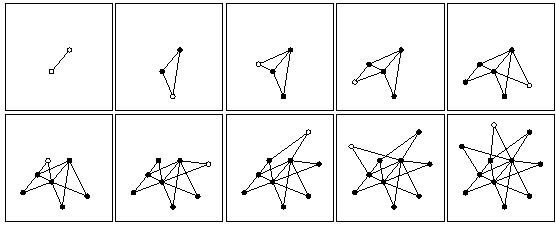
\includegraphics{growth.jpg}}

\columnbreak

%%%Column 3
\section*{Examples of Scale Free Networks}

There are many various examples of Scale Free Networks. These range from Air Traffic Networks to the Internet. Below is an example of a Scale Free network that was generated by the BA algorithm.
\newline
{\centering
\centerline{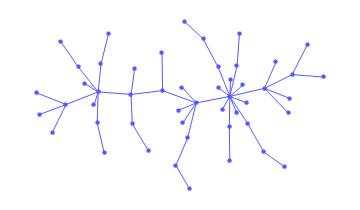
\includegraphics[scale=1.5]{BA.jpg}}}
\newline
The BA network above is created using 50 nodes that each initially had a degree of 1.
After applying the BA algorithm, it is visible there are very few nodes with a high degree. This is due to nodes that have a higher degree have a high probability of gaining more links, thus the "rich" are becoming "richer". This also means that the new network created follows Power Law distribution.
\newline

\centerline{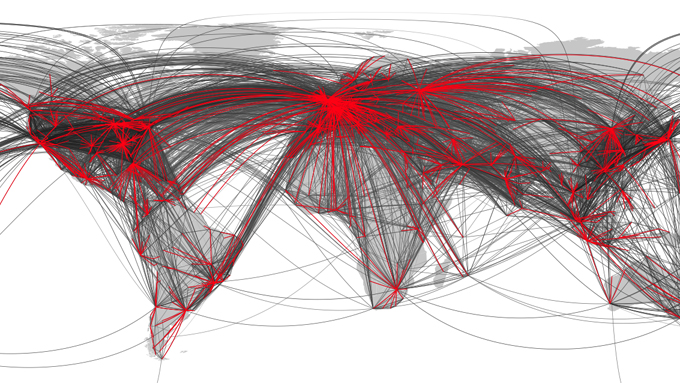
\includegraphics{airtraffic.jpg}}

The figure above shows the Global Air Traffic Network. It shows the there are a few internation airports (nodes) in the world that connect (link) to many different places. However most airports only connect to a small number of places, thus these airports have a small degree. Again this Air Traffic Network has the Power Law Distribution property.

\section*{Conclusion}
In this poster, a Scale Free BA network was defined, An algorithm was presented. Several parameters were introduced. The results were analysed as these parameters vary. There is XX difference when increasing the size of the network and similarities were investigated and compared with small real-world networks. In addition, topological properties were analysed. 
%\nocite*

\bibliographystyle{plain}
\bibliography{halobib}

\end{multicols}
\end{document}
